\documentclass{article}
\usepackage[utf8]{inputenc}
\usepackage{kotex}
\usepackage{verbatim}
\usepackage{graphicx}
\usepackage{subfigure}
\usepackage{indentfirst}
\usepackage{caption}
\usepackage{listings}
\usepackage{xcolor}
\usepackage{geometry}
\geometry{
    a4paper,
    left=30mm,
    right=30mm,
    top=30mm,
    bottom=40mm
}

\lstset{language=C++,
            basicstyle=\ttfamily,
            keywordstyle=\color{blue}\ttfamily,
            stringstyle=\color{red}\ttfamily,
            commentstyle=\color{teal}\ttfamily,
            numberstyle=\tiny\color{gray}\ttfamily,
            morecomment=[l][\color{magenta}]{\#}
            breakatwhitespace=false,         
            breaklines=true,                 
            captionpos=b,                    
            keepspaces=true,                 
            numbers=left,                    
            numbersep=5pt,                  
            showspaces=false,                
            showstringspaces=false,
            showtabs=false,                  
            tabsize=2
}


\title{자료구조 HW5 Postfix}
\author{C211123 이준선}
\date{\today}

\begin{document}
\maketitle

\tableofcontents
\listoffigures
\lstlistoflistings

\section{개요}
Stack 자료구조를 이용하여 중위표기법으로 입력된 수식을 후위표기법(\textit{Postfix})으로 출력하는 프로그램을 구현하였다. 각 피연산자(\textit{Operand})와 연산자(\textit{Operator})를 하나씩 토큰으로 만들고, 이 토큰의 저장과 출력을 선입후출로 대표되는 Stack의 특성과, 연산자 우선순위를 설정하여 관리하였다.
\section{Stack}
\begin{figure} [ht]
    \centering
    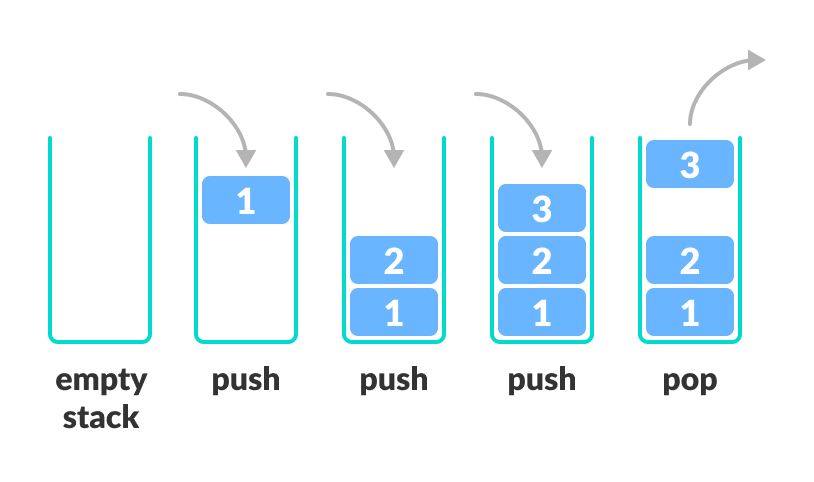
\includegraphics{stack.png}
    \caption{Stack의 개념도}
    \label{fig:concept of stack}
\end{figure}
Stack은 선입후출이란 말로 대표되는 자료구조이다. Figure \ref{fig:concept of stack}을 보면, 스택의 동작 과정에 대해 알 수 있다. 먼저 스택은 push 연산을 통해 데이터를 저장하며, pop연산을 통해 데이터를 빼낸다. Figure \ref{fig:concept of stack}에서 3이 가장 나중에 들어왔지만, 나갈 때는 가장 먼저 나가듯이, 선입후출(\textit{LIFO, Last In, First Out}) 형태를 띄고 있음을 알 수 있다. 한편 가장 위(top)에 있는 자료를 빼내지 않고 보는 연산을 peek이라고 하기도 한다. peek은 top의 자료를 확인하고 꺼내는 pop에서, 꺼내는 과정을 없애고 확인하는 과정만 남긴 형태로 볼 수 있다. 한편 C++에서는 peek 연산이 top()으로 구현되어 있으며, pop()은 빼낸 데이터를 반환하지 않고, void를 반환한다. 그리고 맨 위 데이터를 삭제한다. pop()이 데이터를 반환하지 않음에 주의해야 한다.
\section{Postfix with Stack} \label{Postfix with Stack}
중위표기법을 후위표기법으로 옮기는 연산은 스택을 활용하여 구현될 수 있다. 이는 마치 스택을 쟁반으로 활용하는 것으로 비유할 수 있다. 이 쟁반은 연산자만 담을 수 있는 쟁반이다. 한편 중위표기법의 수식을 중위표기법 입력단, 그리고 이를 후위표기법으로 변환하여 출력이 될 수식이 위치한 자리를 후윞표기법 출력단이라 하자. 예를 들어 5 + 2 / 7 이라는 중위표기법 수식이 중위표기법 입력단에 있다고 하자. 그리고 연산자를 담는 쟁반이 있다. 이 쟁반은 피연산자의 경우 담지 않고, 그대로 후위표기법 출력단으로 넘긴다. 한편 연산자를 만났을 경우, 다음 조건에 따라 쟁반에 담거나, 또는 이미 쟁반에 담긴 연산자들을 pop하여 후위표기법 출력단으로 꺼내 넘긴다. 조건은 다음과 같다.
\begin{enumerate}
    \item 새 연산자가 들어왔을 때, \textbf{쟁반에 이미 위치한 연산자의 우선순위가 높거나 같으면\footnote{이때 연산자 순위가 같아도 높다고 가정함에 유의해야 한다. 예를  들어 $+$, $-$는 동일한 연산자 우선 순위를 가지고 있지만, 쟁반에 $+$가 먼저 담겨 있다고 가정했을 경우, $+$는 연산자 순위가 높다고 가정되어야 한다. 그렇지 않고 $-$ 연산이 $+$ 연산의 스택 위로 쌓였을 경우, 계산 순서가 뒤바뀔 수 있기 때문이다. 즉 연산자 우선 순위가 같을 경우 먼저 들어간 연산자가 우선 순위가 높다고 가정한다.}}
    \begin{itemize}
        \item 쟁반에 위치한 연산자를 꺼내서 변환된 수식이 위치할 자리(후위표기법 출력단)로 옮긴다.
        \item 그리고 새 연산자는 쟁반으로 옮긴다.
    \end{itemize}
    \item 새 연산자가 들어왔을 때, \textbf{쟁반에 위치한 연산자의 우선순위가 낮다면}
    \begin{itemize}
        \item 쟁반에 위치한 연산자의 위에 새 연산자를 쌓는다.
    \end{itemize}
    \item 더 이상 새 연산자가 없으면
    \begin{itemize}
        \item 쟁반에 담긴 연산자를 차례로 pop하여 후위표기법 출력단으로 옮긴다.
    \end{itemize}
\end{enumerate}
위 연산들은 우선순위가 높은 연산자는 우선순위가 낮은 연산자 위에 올라서서, 우선순위가 낮은 연산자가 먼저 자리를 잡지 못하게 하려는 목적을 가지고 있다. 이를 정리하자면 다음과 같이 정리할 수 있다.
\begin{itemize}
    \item 피연산자는 그냥 옮긴다.
    \item 연산자는 쟁반으로 옮긴다.
    \item 연산자가 쟁반에 있다면 우선순위를 비교하여 처리방법을 결정한다.
    \item 마지막까지 쟁반에 남아있는 연산자들은 하나씩 꺼내서 옮긴다.
\end{itemize}
한편 처리해야 할 문제가 하나 더 남아 있는데, 이는 괄호의 처리에 대해서다. 일반적으로 후위표기법에서는 괄호의 표현이 필요하지 않는데, 이는 후위표기법에서는 연산자의 순서 그 자체가 연산 우선 순위를 결정하기 때문이다. 그러나 중위표기법에서는 괄호의 유무로 연산자의 우선 순위가 바뀌기도 한다. 괄호의 처리는 다음과 같이 구성하였다. 먼저 여는 소괄호`('의 쟁반 안에서의 우선순위는 가장 낮게 설정하였다. 그래서 `(' 이후에 연산들을 `(' 위에 쌓을 수 있다. 이후 만약 닫는 소괄호 `)'를 만난다면, 다시 여는 소괄호 `('을 만날 때까지 pop을 통해 후위표기법 출력단으로 옮긴다. 이후 `('을 만나면, `('은 출력하지 않고 pop만 한다\footnote{후위표기법에서 괄호는 필요하지 않기 때문에, 출력하지 아니한다.}. 반면 `('가 들어오는 경우, 이때 `('의 우선순위는 가장 높게 부여하였다. 이럴 경우 `(' 이전에 있던 연산자들을 미리 후위표기법 출력단으로 옮길 수가 있다. 즉 `(' 이전에 존재하는 연산자가 소괄호 안의 연산자와 순서가 섞일 일이 없도록 한다. 여기서는 `(' 연산자의 icp(\textit{in-coming priority})가 가장 높아야 하기에 0으로 설정하였고, isp(\textit{in-stack priority})는 가장 낮아야 하기에, 9로 설정하였다. 이때 9는, 수식의 끝을 의미하는 `\#'의 isp인 10보다는 높은 우선순위를 가지지만, 다른 연산자들보다는 낮은 우선순위를 가진다\footnote{연산자 우선순위의 숫자가 낮을수록(0에 가까울수록) 높은 우선순위를 가지며, 숫자가 클수록(10에 가까울수록) 낮은 우선순위를 가진다.}.

한편 Figure \ref{fig:postfixProcess1}, \ref{fig:postfixProcess2}, \ref{fig:postfixProcess3}, \ref{fig:postfixProcess4}, \ref{fig:postfixProcess5}는 수식 $5 + 2 / 7$을 후치수식으로 변환하는 과정을 보여준다.
\begin{figure} [ht!]
    \centering
    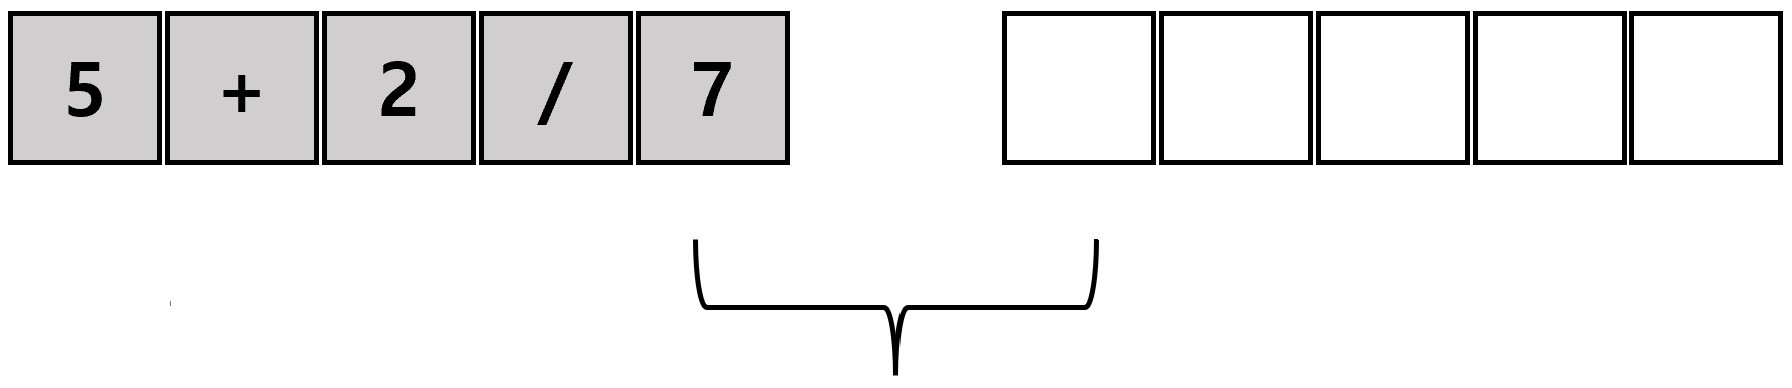
\includegraphics[width=\textwidth]{postfix_process_1.jpg}
    \caption[수식 변환 과정 1]{수식 변환 과정 1. 중위표기법 입력}
    \label{fig:postfixProcess1}
\end{figure}
\begin{figure}[ht!]
    \centering
    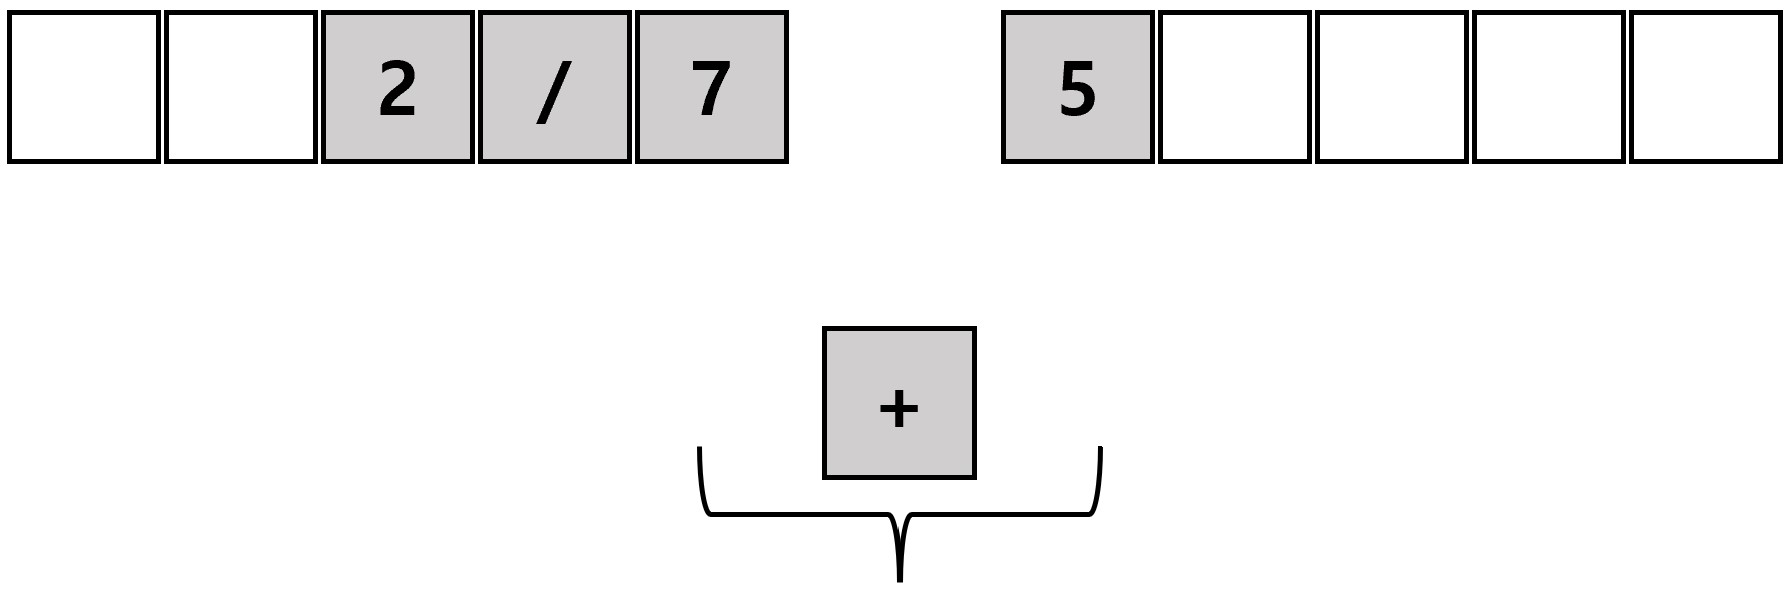
\includegraphics[width=\textwidth]{postfix_process_2.jpg}
    \caption[수식 변환 과정 2]{수식 변환 과정 2. 피연산자인 5는 그대로 출력하고, 연산자인 `$+$'를 쟁반에 담는다}
    \label{fig:postfixProcess2}
\end{figure}
\begin{figure}[ht!]
    \centering
    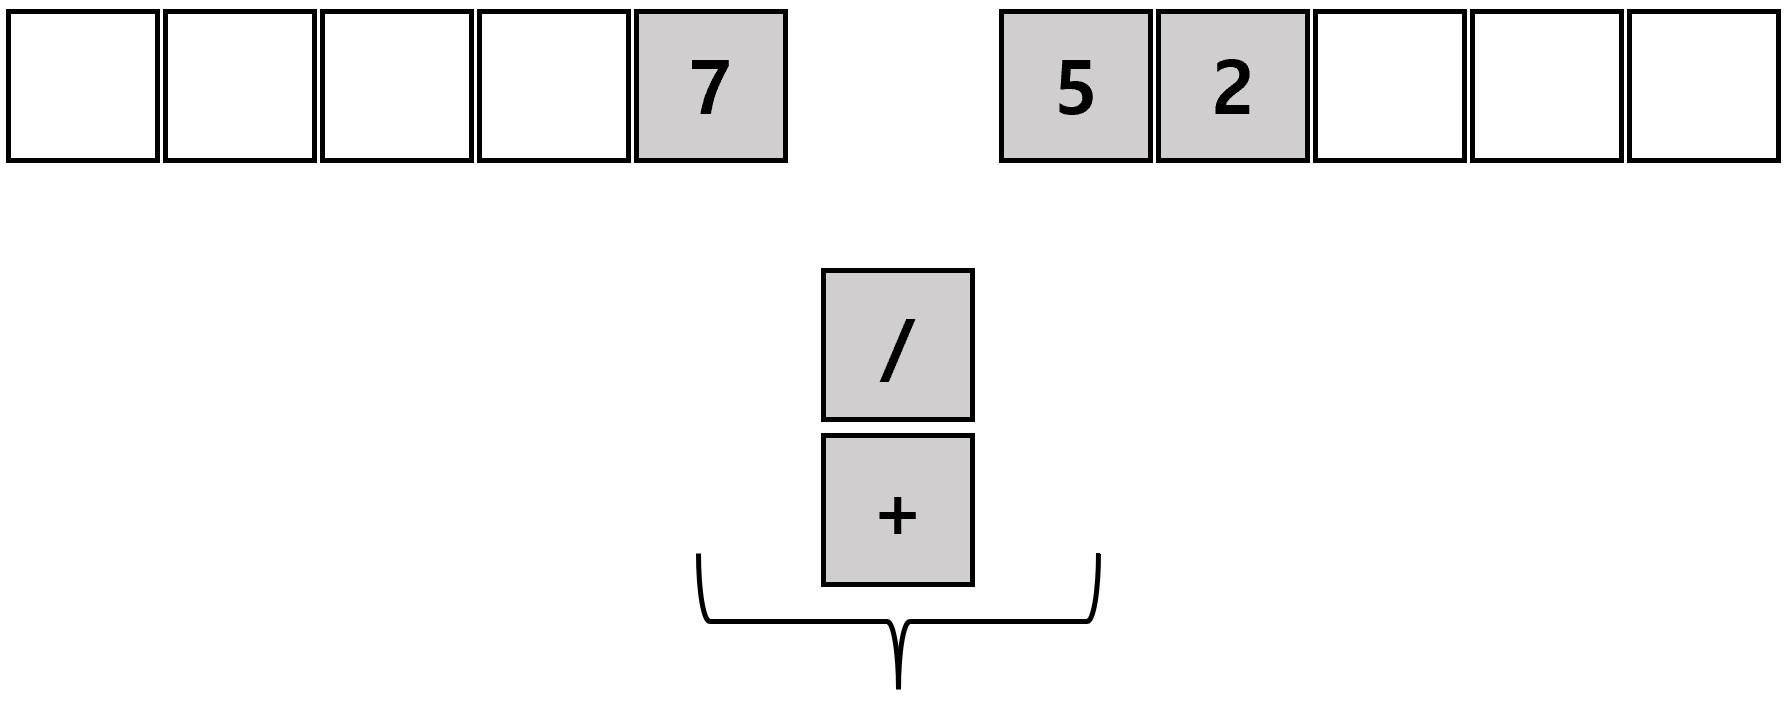
\includegraphics[width=\textwidth]{postfix_process_3.jpg}
    \caption[수식 변환 과정 3]{수식 변환 과정 3. 피연산자인 2는 그대로 출력하고, 연산자 `/'는 `$+$'와의 우선 순위 비교에서 앞서 있기 때문에(\textit{즉 이미 쟁반에 위치한 `$+$'가 우선 순위가 낮기 때문에}) 쟁반 위로 push한다.}
    \label{fig:postfixProcess3}
\end{figure}
\begin{figure}[ht!]
    \centering
    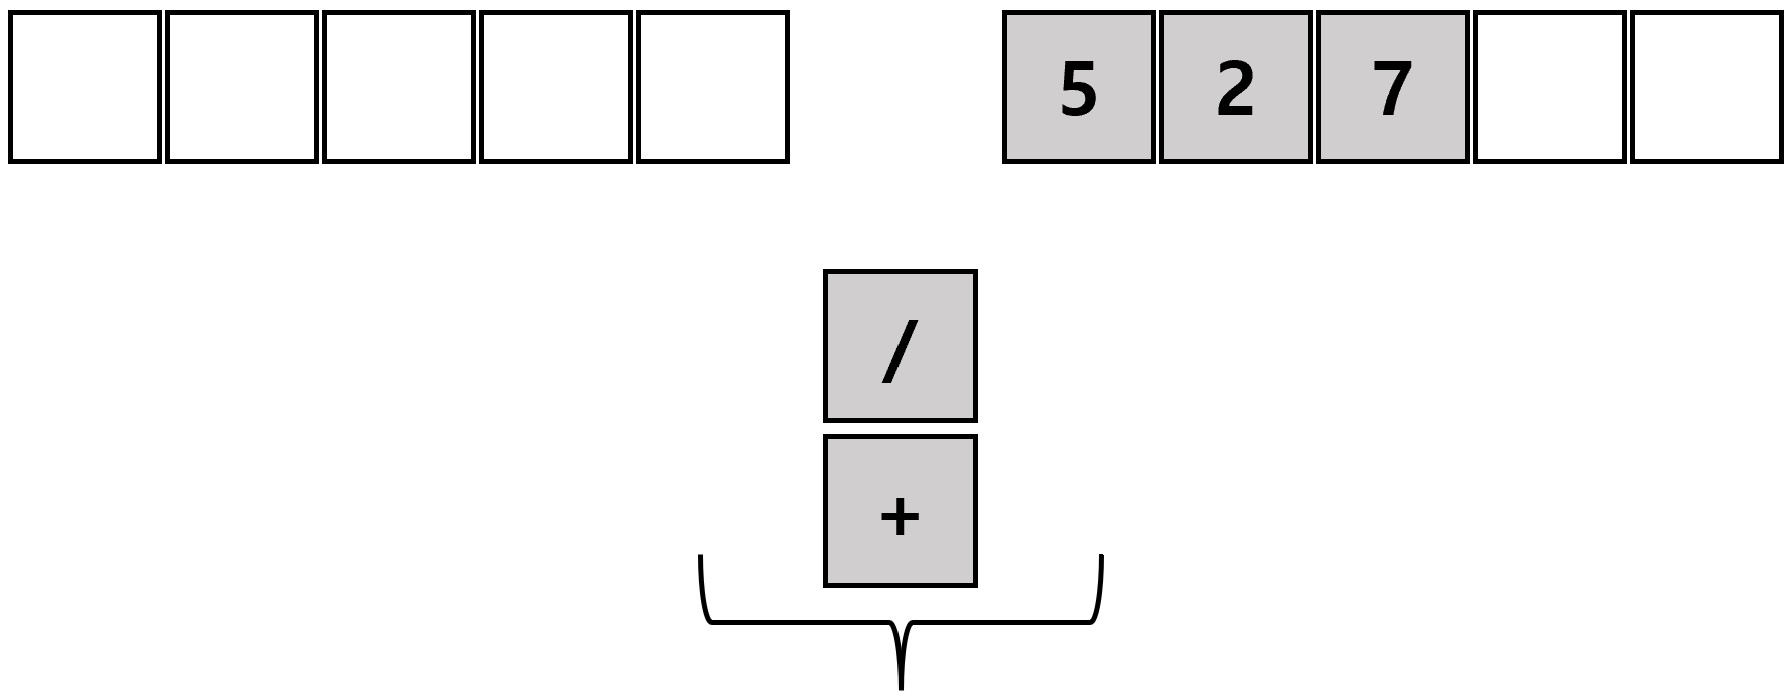
\includegraphics[width = \textwidth]{postfix_process_4.jpg}
    \caption[수식 변환 과정 4]{수식 변환 과정 4. 남은 피연산자인 7은 그대로 출력된다.}
    \label{fig:postfixProcess4}
\end{figure}
\begin{figure}[ht!]
    \centering
    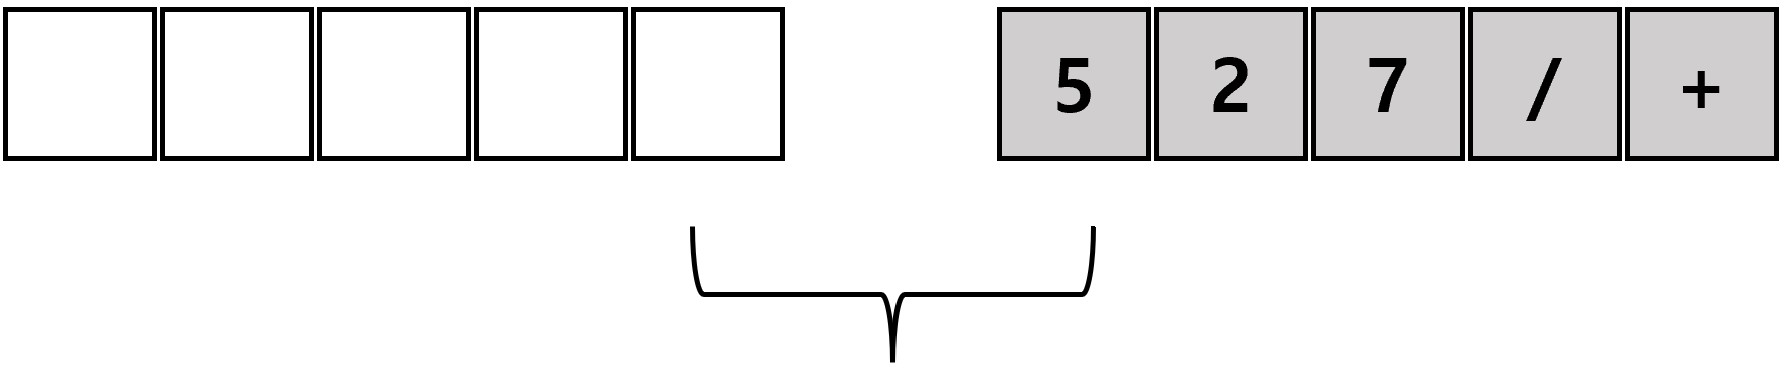
\includegraphics[width = \textwidth]{postfix_process_5.jpg}
    \caption[수식 변환 과정 5]{수식 변환 과정 5. 더이상 남은 중위표기법 입력단이 없기에, 쟁반에서 연산자를 차례로 pop하여 출력한다. `/'가 먼저 pop되어 출력되고, 이후 `$+$'가 pop되어 출력된다.}
    \label{fig:postfixProcess5}
\end{figure}
\section{코드 설명}
\subsection{코드 전문}
\begin{lstlisting} [language=C++, caption=post.h]
#ifndef POSTFIX_H
#define POSTFIX_H
// token types for non one-char tokens
#define ID 257
#define NUM 258
#define EQ 259
#define NE 260
#define GE 261
#define LE 262
#define AND 263
#define OR 264
#define UMINUS 265
#define MAXLEN 80
#define ERROR -1
struct Expression {
	Expression(char* s) : str(s), pos(0)
	{
		for (len = 0; str[len] != '\0'; len++);
	}
	char* str;
	int pos;
	int len;
};
struct Token {
	bool operator==(char);
	bool operator!=(char);
	Token();
	Token(char); // 1-char token: type equals the token itself
	Token(char, char, int); // 2-char token(e.g. <=) & its type(e.g.LE)
	Token(char*, int, int); //operand with its length & type(defaulted to ID)
	bool IsOperand(); // true if the token type is ID or NUM
	int type; // ascii code for 1-char op; predefined for other tokens
	char* str; // token value
	int len; // length of str
	int ival; // used to store an integer for type NUM; init to 0 for ID
};
using namespace std;
ostream& operator<<(ostream&, Token t);
Token NextToken(Expression&, bool); // 2nd arg = true for infix expression
enum OperatorPriority {LEFTBRACKET_icp, UMINUS_FACTORIAL, MULTI_DIVIDE, PLUS_MINUS, LE_GE, EQ_NQ, _AND, _OR, EQUAL, LEFTBRACKET_isp,SHARP = 10};
#endif
\end{lstlisting}

\begin{lstlisting} [language=C++, caption=post.cpp, label={lstlisting:post.cpp}] 
bool GetInt(Expression& e, Token& tok)
{
	char arr[MAXLEN]; int intLen = 0;
	char c = e.str[e.pos];
	if (c < '0' || c > '9') return false; // if c is not integer, return false
	arr[intLen++] = c;
	e.pos++;
	for (c = e.str[e.pos]; '0' <= c && c <= '9'; c = e.str[++e.pos]) {
		arr[intLen++] = c;
	}
	arr[intLen] = '\0';
	tok = Token(arr, intLen, NUM);
	return true;
}

bool TwoCharOp(Expression& e, Token& tok) {
	// handling two char operator token such as <= >= == != && || -u
	char c = e.str[e.pos]; char c2 = e.str[e.pos + 1];
	int op; // LE GE EQ NE AND OR UMINUS
	if (c == '<' && c2 == '=') op = LE;			// <=
	else if (c == '>' && c2 == '=') op = GE;	// >=
	else if (c == '=' && c2 == '=') op = EQ;	// ==
	else if (c == '!' && c2 == '=') op = NE;	// !=
	else if (c == '&' && c2 == '&') op = AND;	// &&
	else if (c == '|' && c2 == '|') op = OR;	// ||
	else if (c == '-' && c2 == 'u') op = UMINUS;
	else { return false; } // if not two char operator, return false
	tok = Token(c, c2, op); e.pos += 2;
	return true;
}

Token NextToken(Expression& e, bool INFIX = true) {
	static bool oprrFound = true; // Assume that operator is previously found
	static bool previousIsBracket = false; // whether last operator was bracket or not
	Token tok;
	SkipBlanks(e); // skip blanks if any
	if (e.pos == e.len) { // No more token left in this expression
		if (INFIX) oprrFound = true; return Token('#');
	}
	if (GetID(e, tok) || GetInt(e, tok)) {
		if (INFIX) oprrFound = false; return tok;
	}
	if(TwoCharOp(e, tok) || OneCharOp(e, tok)) {
		// find '-' after previous was operator 
		if (tok.type == '-' && INFIX && oprrFound && !previousIsBracket) {
			tok = Token('-', 'u', UMINUS); // change into unary minus(-u)
		}
		if (INFIX) oprrFound = true;
		if (tok.type == '(' && INFIX) {
			previousIsBracket = true;
		}
		return tok;
	}
	throw "Illegal Character Found";
}

int icp(Token& t) { // in-coming priority
	int ty = t.type;
	if (ty == '(') return LEFTBRACKET_icp;
	else if (ty == UMINUS || ty == '!') return UMINUS_FACTORIAL;
	else if (ty == '*' || ty == '/' || ty == '%') return MULTI_DIVIDE;
	else if (ty == '+' || ty == '-') return PLUS_MINUS;
	else if (ty == '<' || ty == '>' || ty == LE || ty == GE) return LE_GE;
	else if (ty == AND) return _AND;
	else if (ty == OR) return _OR;
	else if (ty == '=') return EQUAL;
	else if (ty == '#') return SHARP;
	else return ERROR;
}

int isp(Token& t) // in-stack priority
{
	int ty = t.type;
	// in stack, priority of left bracket should be changed into minimum
	// But it should be over than '#'= 10, so 9 is proper one
	if (ty == '(') return LEFTBRACKET_isp;
	else if (ty == UMINUS || ty == '!') return UMINUS_FACTORIAL;
	else if (ty == '*' || ty == '/' || ty == '%') return MULTI_DIVIDE;
	else if (ty == '+' || ty == '-') return PLUS_MINUS;
	else if (ty == '<' || ty == '>' || ty == LE || ty == GE) return LE_GE;
	else if (ty == AND) return _AND;
	else if (ty == OR) return _OR;
	else if (ty == '=') return EQUAL;
	else if (ty == '#') return SHARP;
	else return ERROR;
}

void Postfix(Expression e)
{
	// Print infix expression e as a postfix form
	// If there's no token in e, then return '#' token
	// At the bottom of the stack pushed '#' first
	stack<Token> Stack_Expression;
	Stack_Expression.push('#');
	for (Token x = NextToken(e); x != '#'; x = NextToken(e)) {
		if (x.IsOperand()) cout << x; // if x is an operand, then print x directly
		else if (x == ')') { // if x is rightbracket ')', then unstack until '(' has come
			for (; Stack_Expression.top() != '('; Stack_Expression.pop()) {
				cout << Stack_Expression.top();
			}
			Stack_Expression.pop(); // unstack '('
		}
		else { // x is an operator
			for (; isp(Stack_Expression.top()) <= icp(x); Stack_Expression.pop()) {
				cout << Stack_Expression.top();
			}
			Stack_Expression.push(x);
		}
	}

	// end of expression; empty the stack
	while (Stack_Expression.top() != '#') {
		cout << Stack_Expression.top(); Stack_Expression.pop();
	}
	cout << endl; 
	Stack_Expression.pop();
}
\end{lstlisting}
한편 Listing \ref{lstlisting:post.cpp}은 지면의 분량 관계상 전체 post.cpp가 아닌, assingment 상에서 변경 부분이 있거나 중요한 부분만 기재하였다. 전체 코드는 첨부한 제출한 파일을 참조하라.
\subsection{isp, icp}
isp(\textit{in-stack priority}), icp(\textit{in-comming priority})는 각각 스택 안과 스택 삽입 시의 연산자 우선 순위를 결정하는 함수이다. 연산자 우선순위가 높을수록 0에 가까운 정수를 반환하며, 연산자 우선순위가 낮을수록 10에 가까운 정수를 반환한다. 연산자 우선순위가 가장 낮은 건 \#으로 수식의 끝을 의미하며, 모든 연산자는 \# 위에 차례로 쌓여야 한다.

한편 반환되는 상수는 post.h의 operatorPriority enum으로 관리한다. 각각의 값은 비교 연산에서의 상관 관계만 바뀌지 않는다면 0부터 10까지가 아닌, 어떠한 값이 들어가도 무방하다. 한편 공지된 assignment 안내 자료에서는 \#을 9로 설정하였지만, 여기서는 LEFTBRACKET\_isp(9)의 할당을 위해 10으로 변경하였다.

isp와 icp의 유일한 차이점은 `('의 연산자 우선순위가 다르다는 점 뿐이며, isp에서는 `('에 대해 가장 낮은 우선순위인 9를 반환하지만, icp에서는 `('에 대해 가장 높은 우선순위인 0을 반환한다\footnote{해당 이유에 대해서는 section \ref{Postfix with Stack}의 설명을 참조}.
\subsection{GetInt}
\begin{lstlisting} [language=C++, caption=function getInt()]
bool GetInt(Expression& e, Token& tok)
{
	char arr[MAXLEN]; int intLen = 0;
	char c = e.str[e.pos];
	if (c < '0' || c > '9') return false; // if c is not integer, return false
	arr[intLen++] = c;
	e.pos++;
	for (c = e.str[e.pos]; '0' <= c && c <= '9'; c = e.str[++e.pos]) {
		arr[intLen++] = c;
	}
	arr[intLen] = '\0';
	tok = Token(arr, intLen, NUM);
}
\end{lstlisting}
e.pos에 있는 character가 정수인지 아닌지를 true, false로 반환하고, 이를 토큰으로 저장하는 함수이다. 만약 e.pos에 있는 char가 정수가 아니라면 false를 반환하고, n자리 정수라면 n자리 수를 NUM 형태로 토큰에 저장한다. 이후 e.pos는 정수집합 뒤로 넘겨진다.
\subsection{TwoCharOp}
두 글자 토큰들($<=$, $>=$, $==$, $!=$, \&\&, $||$, $-$u)를 처리하는 함수이다. 이때 $-$u는 단항 연산자 $-$를 의미한다. 두 글자 연산자가 아니면 false를 반환하며, 두 글자 연산자가 맞으면 토큰에 각 연산자에 할당된 상수를 저장한다. 각 상수는 post.h에 할당되어 있다.
\subsection{NextToken}
\begin{lstlisting} [language=C++, caption=function NextToken()]
Token NextToken(Expression& e, bool INFIX = true) {
	static bool oprrFound = true; // Assume that operator is previously found
	static bool previousIsBracket = false; // whether last operator was bracket or not
	Token tok;
	SkipBlanks(e); // skip blanks if any
	if (e.pos == e.len) { // No more token left in this expression
		if (INFIX) oprrFound = true; return Token('#');
	}
	if (GetID(e, tok) || GetInt(e, tok)) {
		if (INFIX) oprrFound = false; return tok;
	}
	if(TwoCharOp(e, tok) || OneCharOp(e, tok)) {
	    // find '-' after previous was operator 
		if (tok.type == '-' && INFIX && oprrFound && !previousIsBracket) {
			tok = Token('-', 'u', UMINUS); // change into unary minus(-u)
		}
		if (INFIX) oprrFound = true;
		if (tok.type == '(' && INFIX) {
			previousIsBracket = true;
		}
		return tok;
	}
	throw "Illegal Character Found";
}
\end{lstlisting}
NextToken의 경우 assingnment 안내서에 공시된 함수 코드와 조금 다르게 작성하였다. 해당 코드로 작성할 경우, 예를 들어 다음 입력에 대해 다음 출력 결과를 나타낸다.
입력 : $3 / (2 + 7) - 5$
출력 : $3 2 7 + / 5 -u$
이는 단항 $-$연산자 UMINUS를 인식하는 방식이, 기존의 경우 operator가 발견된 직후 다시 $-$가 발견되었을 경우, 이를 단항 연산자 UMINUS로 처리하였기 때문이다. 그러나 괄호는 연산자이나 후위표기법에서는 출력되지 않기에, 괄호 바로 뒤에 $-$가 올 경우 문제가 발생한다. 즉 괄호 뒤에 온 $-5$의 경우 $5 -u$로 처리되면 안 되고, 정상적으로 MINUS 연산으로 처리되어야 한다. 때문에 previousIsBracket이라는 bool형 변수를 만들어 이 문제를 해결했다. 즉 이전 연산자가 여는 소괄호 `('가 아닌 경우에만 연산자 이후 발견된 $-$에 대해 UMINUS 처리를 하겠다는 뜻이다. 이럴 경우 정상적으로 괄호 바로 뒤에 입력된 $-$에 대해 MINUS로 인식할 수 있게 된다.
\subsection{Postfix}
\begin{lstlisting} [language=C++, caption=function Postfix()]
void Postfix(Expression e)
{
	// Print infix expression e as a postfix form
	// If there's no token in e, then return '#' token
	// At the bottom of the stack pushed '#' first
	stack<Token> Stack_Expression;
	Stack_Expression.push('#');
	for (Token x = NextToken(e); x != '#'; x = NextToken(e)) {
		if (x.IsOperand()) cout << x; // if x is an operand, then print x directly
		else if (x == ')') { // if x is rightbracket ')', then unstack until '(' has come
			for (; Stack_Expression.top() != '('; Stack_Expression.pop()) {
				cout << Stack_Expression.top();
			}
			Stack_Expression.pop(); // unstack '('
		}
		else { // x is an operator
			for (; isp(Stack_Expression.top()) <= icp(x); Stack_Expression.pop()) {
				cout << Stack_Expression.top();
			}
			Stack_Expression.push(x);
		}
	}

	// end of expression; empty the stack
	while (Stack_Expression.top() != '#') {
		cout << Stack_Expression.top(); Stack_Expression.pop();
	}
	cout << endl; 
	Stack_Expression.pop();
}
\end{lstlisting}
Postfix 함수의 경우 교재를 다수 참고하였다. 기본 원리는, Token x 에다가 `\#'이 아닐 때까지 계속해서 다음 토큰을 담는다. 이후 x가 피연산자이면 그대로 출력하고, x가 `)'(닫는 괄호)일 경우 `('(여는 괄호)가 나올 때까지 기존 연산자가 담긴 Stack\_Expression의 연산자들을 모두 pop하여 출력한다. x가 연산자일 경우, 연산자 우선순위 비교에 따라 Stack\_Expression에 그대로 push하거나 기존에 있던 연산자들을 모두 pop하여 출력한 후 push한다.
\begin{lstlisting} [language=C++, caption=loop]
for (; isp(Stack_Expression.top()) <= icp(x); Stack_Expression.pop()) {
		cout << Stack_Expression.top();
}
\end{lstlisting}
위 반복문이 Stack\_Expression 안의 isp와 x와의 icp(우선순위) 비교를 통해 출력을 할 지 그대로 push할 지를 결정한다.
\subsection{main}
\begin{lstlisting} [language=C++, escapeinside=``, caption=main]
int main() {
	char line[MAXLEN];
	cout << "C211123 LEE JUNSEON, `이준선`" << endl;
	while (cin.getline(line, MAXLEN)) {
		Expression e(line); // reading expression using line buffer
		try {
			Postfix(e);
		}
		catch (char const* msg) {
			cerr << "Exception: " << msg << endl;
		}
	}
}
\end{lstlisting}
한편 main함수의 경우 위와 같다.
assingnment 안내서에 고지된 바와 같이 학번과 이름\footnote{Linux 환경에서 한글이 지원되지 않아 Linux 환경에서 실행 시 한글 이름이 잘못 출력될 수 있다.}이 출력되게끔 하였으며, 입력 함수의 경우 cin.getline() 함수를 사용하였다.
\section{실행 결과}
\begin{figure} [ht]
    \begin{center}
    \subfigure[post1 result]{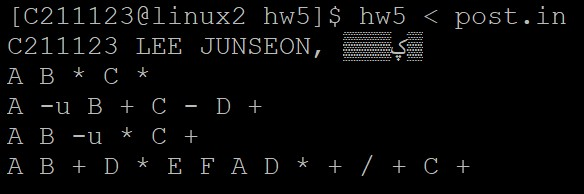
\includegraphics[width=0.8\textwidth]{post_result.jpg}}
    \subfigure[post2 result]{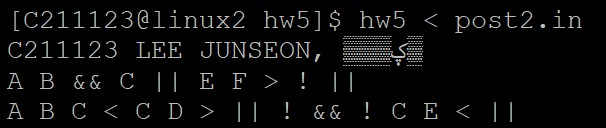
\includegraphics[width=0.8\textwidth]{post2_result.jpg}}
    \subfigure[post3 result]{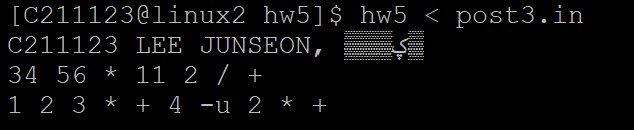
\includegraphics[width=0.8\textwidth]{post3_result.jpg}}
    \subfigure[post4 result]{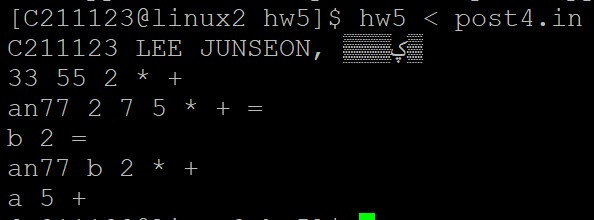
\includegraphics[width=0.8\textwidth]{post4_result.jpg}}
    \caption{실행 결과}
    \label{fig:test result}
    \end{center}
\end{figure}
Figure \ref{fig:test result}는 각각 실행 파일 post1\footnote{assingnment 안내서에서는 post.in, post2.in, post3.in, post4.in 파일을 정의하였다. 이때 post.in 파일은 post1.in 파일로 이해하는 것이 자연스럽다. 때문에 본 글에서 post.in과 post1.in 은 같은 실행 파일을 의미하며, 통일성을 위해 post.in을 post1.in으로 표현하였다.}, post2, post3, post4의 실행결과를 보여준다. 모든 입력 case에 대해 정상적으로 후위표기법으로 변환되어 출력된 것을 확인할 수 있다.

\end{document}
